%------------------------------------
% Chunhua Shen's Publications in LaTeX
% Using the template from http://nitens.org/taraborelli/cvtex
%------------------------------------
%!TEX TS-program = lualatex
%!TEX encoding = UTF-8 Unicode


\documentclass[9pt, a4paper]{article}
\usepackage[T1]{fontenc}
\usepackage{lmodern}
\usepackage{amssymb,amsmath}

\usepackage{graphicx}


\usepackage{ifxetex,ifluatex}
\usepackage{fixltx2e} % provides \textsubscript
% use upquote if available, for straight quotes in verbatim environments
\IfFileExists{upquote.sty}{\usepackage{upquote}}{}
\ifnum 0\ifxetex 1\fi\ifluatex 1\fi=0 % if pdftex
  \usepackage[utf8]{inputenc}
\else % if luatex or xelatex
  \usepackage{fontspec}
  \ifxetex
    \usepackage{xltxtra,xunicode}
  \fi
  \defaultfontfeatures{Mapping=tex-text,Scale=MatchLowercase}
  \newcommand{\euro}{€}
\fi
% use microtype if available
\IfFileExists{microtype.sty}{\usepackage{microtype}}{}


% DOCUMENT LAYOUT

\usepackage[top=.5in, bottom=.5in, left=1.36in, right=1in]{geometry}
\geometry{a4paper, textwidth=5.5in, textheight=8.5in, marginparsep=7pt, marginparwidth=.6in}


\setlength\parindent{0in}




\usepackage[]{metalogo}

% FONTS

\usepackage{xunicode}
\usepackage{xltxtra}
\defaultfontfeatures{Ligatures=TeX} % converts LaTeX specials (``quotes'' --- dashes etc.) to unicode
\setromanfont[Ligatures={Common},Numbers={OldStyle}]{Adobe Caslon Pro}
%\setromanfont[Ligatures={Common}, Numbers={OldStyle}, Variant=01]{Linux Libertine O}
%\setromanfont[Ligatures={Common},Numbers={OldStyle}]{Adobe Garamond Pro}

\setmonofont[Scale=0.7]{Monaco}
%\setsansfont[Scale=0.9]{Lato}
\setsansfont[Mapping=tex-text,Scale=0.8]{Calibri}

% ---- CUSTOM AMPERSAND
\newcommand{\amper}{{\fontspec[Scale=.8]{Adobe Caslon Pro}\selectfont\itshape\&}}


% ---- MARGIN YEARS
\usepackage{./marginnote}

\newcommand{\years}[1]{\marginnote{\scriptsize #1}}
\renewcommand*{\raggedleftmarginnote}{}
\setlength{\marginparsep}{7pt}
\reversemarginpar

\let\id\years


% HEADINGS
\usepackage{sectsty}
\usepackage[normalem]{ulem}
\sectionfont{\rmfamily\mdseries\Large}
\subsectionfont{\rmfamily\mdseries\scshape\normalsize}
\subsubsectionfont{\rmfamily\bfseries\upshape\normalsize}

\usepackage{xcolor}
\usepackage[]{ulem}
\def\highlight{\uline}


\usepackage{bashful}

\usepackage{microtype}
% ----------------------------------------------------------------------
%  \now  -- Current time in h:mm AM/PM format
%  \mdyy -- Today's date in m/d/yy format.  Forget Y2K; this is for humans!
% ----------------------------------------------------------------------
\newcount\timehh\timehh=\time
\divide\timehh by 60
\newcount\timemm\timemm=\time
\count255=\timehh
\multiply\count255 by -60
\advance\timemm by \count255
\newif\iftimePM
\ifnum\timehh>11 \timePMtrue\else\timePMfalse\fi
\ifnum\timehh<1 \advance\timehh by 12\fi
\ifnum\timehh>12 \advance\timehh by -12\fi
\def\now{\number\timehh:\ifnum\timemm<10 0\fi\number\timemm
         \iftimePM {$\,$pm.}  \else {$\,$am.}  \fi}
\newcount\mdYY\mdYY=\year
\count255=\year
\divide\count255 by 100
\multiply\count255 by 100
\advance\mdYY by -\count255
\def\mdyy{\number\month/\number\day/\ifnum\mdYY<10 0\fi\number\mdYY}

% \edef\today{\number\day\space
% \ifcase\month\or
% Jan.\or Feb.\or Mar.\or Apr.\or May\or Jun.\or Jul.\or Aug.\or Sep.\or Oct.\or Nov.\or Dec.\fi, \number\year}
\edef\today{\number\day$\cdot$\number\month$\cdot$\number\year}



\hyphenpenalty=1750
\hyphenation{con-vo-lu-t-i-o-n-a-l cro-ss-con-vo-lu-t-i-on-al-l-a-y-er D-I-C-T-A  C-V-P-R   I-C-C-V}




% PDF SETUP
% ---- FILL IN HERE THE DOC TITLE AND AUTHOR
\usepackage[bookmarks, colorlinks, breaklinks, pdftitle={Chunhua Shen - vita},pdfauthor={Chunhua Shen}]{hyperref}
\hypersetup{linkcolor=blue,citecolor=blue,filecolor=black,urlcolor=blue}

\usepackage[]{marvosym}
\newcommand{\marvosymbol}[1]{{\fontfamily{mvs}\fontencoding{U}\fontseries{m}\fontshape{n}\selectfont\char#1}}
\newcommand{\mobilesymbol}{{\color{red}{\marvosymbol{72}}}~}
\newcommand{\mobile}[1]{\mobilesymbol{#1}}

\newcommand{\phonesymbol}{{\color{red}{\marvosymbol{84}}}~}
\newcommand{\phone}[1]{\phonesymbol{#1}}

\newcommand{\faxsymbol}{{\color{red}{\marvosymbol{117}}}~}
\newcommand{\faxnum}[1]{\faxsymbol{#1}}

\newcommand{\emailsymbol}{{\color{red}{\marvosymbol{66}}}~}
\newcommand{\email}[1]{\emailsymbol{#1}}

\newcommand{\wwwsymbol}{{\color{red}{\marvosymbol{205}}}~}
\newcommand{\web}[1]{\wwwsymbol{\hspace{0.06cm}#1}}

\newcommand{\sepcirc}{\hspace{.02cm}$\color{red}\cdot$\hspace{.1cm}}
\let\and\sepcirc


\usepackage{ifthen,xspace}
\newcommand{\decoauthor}[1]{\ifthenelse{\equal{#1}{}}{Empty author.}{{#1}}}
\newcommand{\decoyear}[1]{\ifthenelse{\equal{#1}{}}{Empty year.}{{(#1),}}}
\newcommand{\decotitle}[1]{\ifthenelse{\equal{#1}{}}{Empty title.}{{ ``#1'',}}}
\newcommand{\decojournal}[1]{\ifthenelse{\equal{#1}{}}{Empty journal.}{\emph{#1}}}
\newcommand{\decovolume}[1]{\ifthenelse{\equal{#1}{}}{}{{ #1}}}
\newcommand{\decopage}[1]{\ifthenelse{\equal{#1}{}}{.}{{: #1.}}}

\newcommand{\decoconf}[1]{\ifthenelse{\equal{#1}{}}{Empty Conference.}{In: \emph{Proc.\ #1}}}

%
% Elements of Typographic Style, recommends to use upright parentheses in italic text
% xparse allows us to easily define \emph to do what you asked for, and \emph* to do the old version of \emph
%
\usepackage{expl3,xparse}
\ExplSyntaxOn
\cs_new_eq:Nc \emph_old:n { emph~ } % Copying the old definition of `\emph`
\cs_new_eq:NN \emph_braces:n \textup % Set up how braces should be typeset.
\cs_new:Npn \emph_new:n #1 {
  \tl_set:Nn \l_emph_tl {#1}
  \tl_replace_all:Nnn \l_emph_tl {(}{\emph_braces:n{(}}
  \tl_replace_all:Nnn \l_emph_tl {)}{\emph_braces:n{)}}
  \tl_replace_all:Nnn \l_emph_tl {[}{\emph_braces:n{[}}
  \tl_replace_all:Nnn \l_emph_tl {]}{\emph_braces:n{]}}
  \exp_args:NV \emph_old:n \l_emph_tl
}
\RenewDocumentCommand {\emph} {sm} {
  \IfBooleanTF {#1} {\emph_old:n {#2}} {\emph_new:n {#2}}
}
\ExplSyntaxOff

\pagestyle{empty}

%
% You should not modify above content; which defines the looking
%


% DOCUMENT
\begin{document}

% {\LARGE  Chunhua Shen}
% \\[.2cm]


\section*{Refereed Publications (\input{bin/num_total.text}\unskip)}

\subsection*{Refereed journal articles (\input{bin/num_journals.text}\unskip)}
\noindent
\input bin/journal.text






%-----------------PART 1: CVPR, ICCV, ECCV, ICML, NeurIPS ------------------------------

\vspace{-0.15cm}
\subsection*{Refereed top conference articles in computer vision and machine learning (\input{bin/num_confs_select.text}\unskip)
}
{
\begin{itemize}
  \itemsep -.12cm
\footnotesize
\item \emph{  Proc.\ Annual Conf.\ Neural Information Processing Systems (NeurIPS)}
\item \emph{  Proc.\ Int.\ Conf.\ Machine Learning (ICML)}
\item \emph{  Proc.\ IEEE Conf.\ Computer Vision \& Pattern Recognition (CVPR)}
\item \emph{  Proc.\ Int.\ Conf.\ Computer  Vision (ICCV)}
\item \emph{  Proc.\ European Conf.\ Computer Vision (ECCV)}
\end{itemize}
}


\noindent
\input bin/conf_selected.text






%-----------------PART 2: AAAI, IJCAI, ICRA  ------------------------------


\vspace{-0.15cm}
\subsection*{Refereed major conference articles in artificial intelligence and robotics (\input{bin/num_confs_select2.text}\unskip)
}
{
\begin{itemize}
  \itemsep -.12cm
\footnotesize
\item \emph{  Proc.\ AAAI Conf.\ Artificial Intelligence (AAAI)}
\item \emph{  Proc.\ Int.\ Joint Conf.\ Artificial Intelligence (IJCAI)}
\item \emph{  Proc.\ ACM SIGKKD Conf.\   Knowledge Discovery and Data Mining (KDD)}
\item \emph{  Proc.\ IEEE Int.\ Conf.\    Robotics \&  Automation (ICRA)}
\item \emph{  Proc.\ British Machine Vision Conf.\ (BMVC)}
\item \emph{  Proc.\ ACM Int.\  Conf.\  Multimedia\ (ACM MM)}
\item \emph{  Proc.\ Int.\ Conf.\ Medical Image Computing and Computer Assisted Intervention (MICCAI)}

\end{itemize}
}




\noindent
\input bin/conf_selected2.text





\vspace{-0.15cm}
\subsection*{Refereed other miscellaneous  conference articles (\input{bin/num_confs_other.text}\unskip)}
\noindent
\input bin/conf_other.text








% Google citation
\subsection*{\href{https://scholar.google.com/citations?hl=en&user=Ljk2BvIAAAAJ&view_op=list_works}{Google scholar citation} ({\it h-index}:  \input{../bin/gcitation_HIndex.text}\unskip; {\it citations}: \input{../bin/gcitation_num.text}\unskip) }

\begin{figure}[h!]
\centering
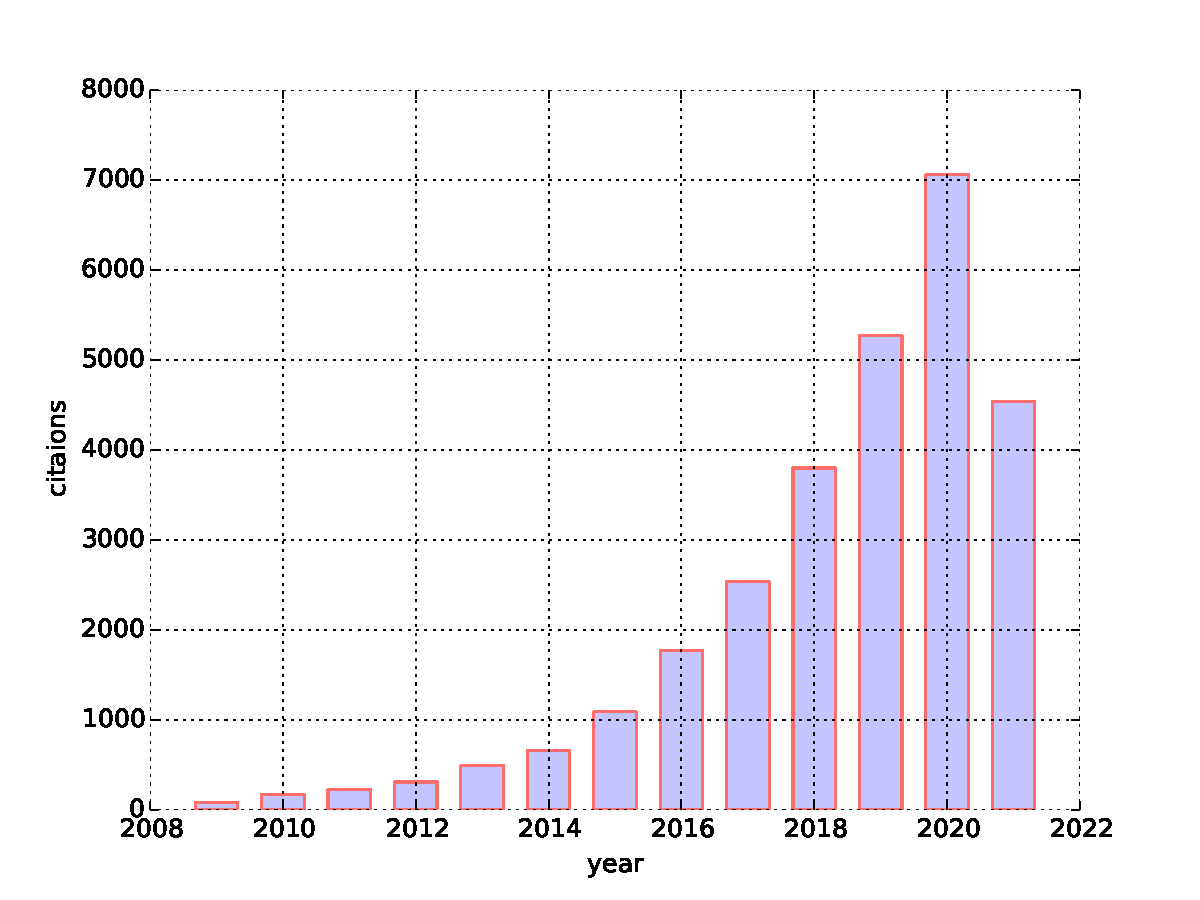
\includegraphics[width=.605\textwidth]{../data/cs_cite}
\caption{Google scholar citation as of \today}
\label{fig:google_scholar}
\end{figure}








\vfill{}
%\hrulefill
\begin{center}
{\scriptsize    Compiled at: \now \today\- •\- Typeset in {
\fontspec{Times New Roman}\XeLaTeX{}
using Python script
}\\
% ---- FILL IN THE FULL URL TO YOUR CV HERE
\href{https://cshen.github.io}{cshen.github.io}
}
\end{center}

\end{document}




